\subsection{MEX 2-3: Effect of compressibility on pressure driven percolation}

Data management for MEX 2-3 (see \ref{sec:mex04}).

\subsubsection*{CAU Kiel}

The required LEM code and the input variables for simulating the effect of compressibility are uploaded to the IfG (Kiel) NextCloud server. The data is accessible through the following link:\\
\hyperlink{https://nextcloud.ifg.uni-kiel.de/index.php/s/6Mfg3P4PyKNN6By}{https://nextcloud.ifg.uni-kiel.de/index.php/s/6Mfg3P4PyKNN6By}\\

The uploaded protected MATLAB file in a *.p format requires a MATLAB version with a built-in Voronoi Tessellation and Delaunay Triangulation functions. The input variables are prepared in two different files for the simulation of the pressure drop in gas and brine reservoirs. Fig. \ref{fig:Amir_ME4_Pressure_Data} shows the differences between the pressure drop in gas and brine reservoirs.

\begin{figure}[!ht]
\centering
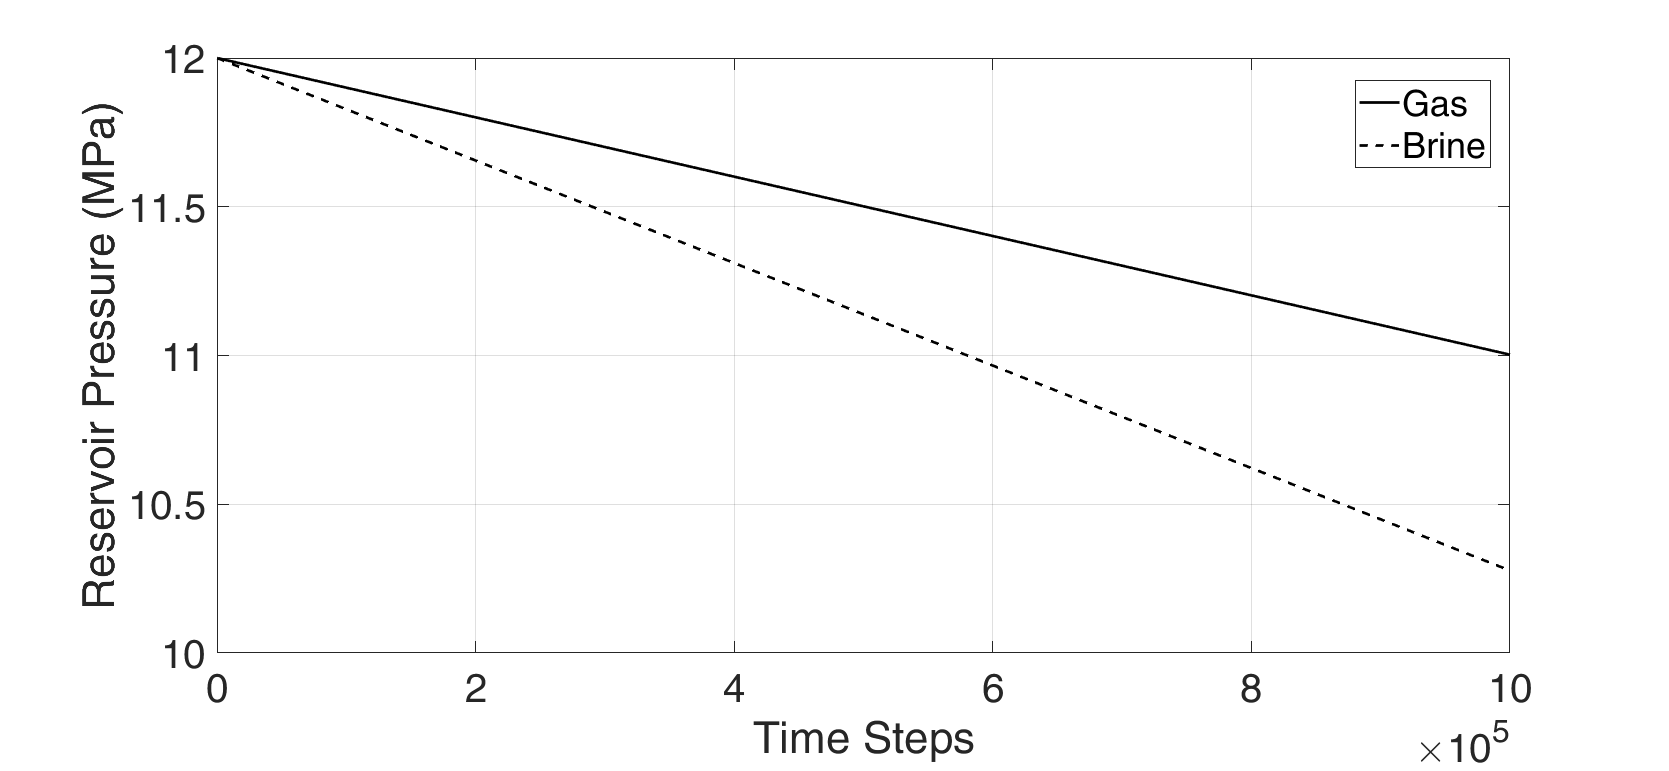
\includegraphics[width=8cm,height=5cm]{figures/Amir_ME4_Pressure_Data.png}
\caption{The comparison between the pressure drop in gas and brine reservoirs}
\label{fig:Amir_ME4_Pressure_Data}
\end{figure}


\begin{table}[!ht]
\caption{MEX 2-3: Effect of compressibility}
\label{tab:dms-mex2-3}
\small
\begin{tabular}{R{3cm}|L{7cm}}
\hline
%
Data label & GeomInt | CAU | Percolation test, effect of compressibility\\
URI &  https://nextcloud.ifg.uni-kiel.de/index.php/s/6Mfg3P4PyKNN6By (Numerics)
\\
Subject  &  Effect of compressibility\\
Type of data  & Executable MATLAB P-file, Input parameters\\
Dataquality  &  quality assured data \\
Status of data  &  unprocessed data\\
Dataformat  & txt, MATLAB executable P-file\\
Creators  &  Kiel University, Institute of Geomechanics and Geotechnics, Ludewig-Meyn-Stra\ss e 10, 24118, Kiel\\
Source/Origin & In-house code \\
Publisher  &  Kiel University, Institute of Geomechanics and Geotechnics, Ludewig-Meyn-Stra\ss e 10, 24118, Kiel \\
Rights holders &  Kiel University, Institute of Geomechanics and Geotechnics, Ludewig-Meyn-Stra\ss e 10, 24118, Kiel \\
Contributors &   Kiel University, Institute of Geomechanics and Geotechnics: Amir Shoarian Sattari, Frank Wuttke\\
Time or Period of creation &  2019-2020\\
Language of the content &  English\\
Update policy &  stored data is final\\
Access permissions & full access\\
%
\hline
\end{tabular}
\end{table}


\todo[inline]{[IfG et al.]: Please add data management info for MEX 2-3}

\begin{table}[!ht]
\caption{MEX 2-3: Meta Data according to Dublin Core}
\label{tab:dms-mex2-3}
\small
\begin{tabular}{R{3cm}|L{7cm}}
\hline
%
Data label &  \\
URI &  \\
Subject  &  \\
Type of data  &  \\
Dataquality  &  \\
Status of data  &  \\
Dataformat  & \\
Creators  &  \\
Source/Origin &  \\
Publisher  &  \\
Rights holders &  \\
Contributors &  \\
Time or Period of creation &  \\
Language of the content &  \\
Update policy &  \\
Access permissions &  \\
%
\hline
\end{tabular}
\end{table}